\documentclass[10pt,journal,compsoc]{IEEEtran}

\usepackage[T1]{fontenc}
\usepackage[utf8]{inputenc}
\usepackage{graphicx}
\usepackage{booktabs}
\usepackage{amsmath}
\usepackage{xcolor}
\usepackage{url}
\usepackage[hidelinks]{hyperref}
\usepackage{cite}

\newcommand{\todo}[1]{\textcolor{red}{\textbf{[TODO: #1]}}}

\begin{document}
\setlength{\tabcolsep}{2.5pt}

\title{Forecasting the Carbon Intensity of California Grid Electricity: An Individual Report on the Data Pipeline}

\author{Jayanth~Naga~Sai~Pasupulati
\thanks{J. N. S. Pasupulati is a student in the Master of Science in Applied Data Intelligence (MSADI) program, San Jose State University, San Jose, CA, USA. Course: DATA 245, Fall 2026. Team members and roles, from the team's role description: Aryan (carbon-intensity forecasting, regression and gradient boosting models) and Jaskirat (day-type clustering and load-shifting simulation). The checklists refer to the modeling roles as M2 and M3, but the role description does not assign those labels, so the mapping of labels to people is not stated here.}}

\markboth{DATA 245 Final Project Report, Fall 2026}{Pasupulati: Carbon Intensity Forecasting Data Pipeline}

\maketitle

\begin{abstract}
The carbon intensity (CI, in gCO$_2$eq/kWh) of electricity varies by hour with the mix of generators that run. This report documents the data pipeline I built for a three-person team project that forecasts the CI of the California Independent System Operator (CAISO) balancing area. The pipeline converts raw hourly grid data from the U.S. Energy Information Administration (EIA-930), nameplate capacity from EIA-860, and NOAA daily and hourly weather into a checksummed feature table for 2019-2025. The headline model forecasts CI 168 hours (7 days) ahead using only information available at forecast time. It uses no weather, because the project has no forecast weather. Two leakage safeguards, a no-future perturbation check and a positive control, each pass on 40 of 40 sampled timestamps for both tables. A gradient boosting model is compared with a seasonal 4-week average and 168-hour persistence using 74 weekly rolling origins on the July 2024 to December 2025 test period. For the lifecycle target the model's mean absolute error (MAE) is 34.97 gCO$_2$eq/kWh, against 36.66 for the seasonal baseline and 41.15 for persistence. The model is better on the pooled test set, but at the level of individual weeks the advantage is small. It beats the seasonal baseline in 40 of 74 folds, and a 95\% bootstrap interval for the mean per-fold difference includes zero. Most of the advantage comes from 2024 origins, and in 2025 the two methods are close to tied. A single fit trained only on the training period does worse than the seasonal baseline. A secondary 1-hour model reaches an MAE of 11.42, which mostly reflects how slowly CI changes from hour to hour. The report describes the data quality problems, the decisions made in response, the verification steps, what was learned, the threats to validity, and the items still open.
\end{abstract}

\begin{IEEEkeywords}
Carbon intensity, electricity grid, time series forecasting, rolling-origin evaluation, data leakage, gradient boosting, reproducible data pipelines.
\end{IEEEkeywords}

\section{Introduction}
\IEEEPARstart{E}{lectricity} is not equally carbon-intensive at all hours. The mix of generators that run to meet demand changes with the time of day, the season, weather, and the availability of hydro, solar, and wind power. A kilowatt-hour drawn at 2 a.m. in spring can carry very different emissions from one drawn at 7 p.m. in late summer. Forecasting this carbon intensity, measured as grams of carbon dioxide equivalent per kilowatt-hour (gCO$_2$eq/kWh), could help users and operators decide when electricity is cleaner. Whether a forecast is useful depends first on whether its inputs are clean. A forecast that quietly uses information from after its forecast time looks far better than it is.

This report covers my part of a three-person team project on CAISO. I was responsible for the M1 data pipeline. The work included acquiring the raw data, verifying it, cleaning it, computing the carbon intensity target, building the input features, enforcing the rule that no feature may use future information, and handing a frozen, checksummed table to the two modeling teammates. The modeling work of the M2 and M3 teammates is described only where it touches the pipeline.

The report has three goals. The first is to document what the pipeline does and why it makes each decision, in enough detail that the results can be checked. The second is to report the evaluation honestly, including the unfavorable parts: the advantage over a seasonal baseline is small, and at the level of individual weeks it is not statistically distinguishable from zero. The third is to record what I learned, the technical difficulties I met, and the practices I would repeat.

The report addresses four questions. (1) Can the raw grid and weather data be turned into a table whose every input is available at forecast time, and can that be checked? Section~\ref{sec:methods} and Table~\ref{tab:splits} answer this, and the no-future check answers the checking part. (2) Does a gradient boosting model with lagged and calendar features beat a seasonal 4-week average and persistence on the test period? Section~\ref{sec:results} answers this, with the pooled result, the fold-level result, and the test-period split. (3) Does the answer depend on the target definition or on the horizon? The combustion-only sensitivity and the 1-hour model address this, and they show that the answer for the combustion target is similar and that a 1-hour forecast is much easier. (4) What would a team need to know before relying on these results? Sections~\ref{sec:discussion} to \ref{sec:limits} answer this. In short, the answers are: yes for the pipeline, a small and inconsistent advantage for the model, similar results for the two targets, and a need for uncertainty to be reported with any claim.

The main contributions of my part are: (1) a one-command pipeline that rebuilds a feature table from raw files, with a SHA-256 manifest and a read-only raw data store; (2) a carbon intensity target built from generation by fuel and lifecycle emission factors, with a combustion-only sensitivity version; (3) a leakage control with a positive control, so that the check can fail; (4) a rolling-origin evaluation that refits the model at each of 74 weekly origins, with fold-level uncertainty; and (5) a verification record covering data quality findings, a station-name discrepancy I identified, and environment problems that were fixed or documented.

Section~\ref{sec:related} places the work in context. Section~\ref{sec:data} describes the data, Section~\ref{sec:methods} the methods, Section~\ref{sec:results} the results, Section~\ref{sec:discussion} the interpretation, Section~\ref{sec:threats} the threats to validity, Section~\ref{sec:learn} the learning outcomes, and Section~\ref{sec:limits} the limitations. Section~\ref{sec:course} relates the work to the course. Appendices give the rubric evidence, the tools used, and the files and links.

\section{Background and Related Work}
\label{sec:related}

\subsection{Carbon intensity and its definitions}
The carbon intensity of electricity is the emissions of the generation mix divided by the energy it produces. Two definitions appear in the literature and in this project. A \emph{combustion-only} definition counts only the direct emissions at the plant. A \emph{lifecycle} definition adds upstream emissions, such as fuel extraction and transport, and emissions from building the plant. The IPCC Fifth Assessment Report gives lifecycle emission estimates for each generation technology as ranges and medians \cite{ipcc2014}. The project uses the medians for its headline target. The combustion-only definition is a sensitivity analysis. Its factors come from heat rates and default carbon dioxide content per unit of fuel energy \cite{ipcc2006}. They are assumptions rather than a sourced table, as Section~\ref{sec:methods} explains.

\subsection{Forecasting and evaluation}
Time-series forecasting is usually judged against simple baselines. Persistence, which forecasts the value observed one period earlier, and seasonal naive methods, which forecast the value observed one season earlier, are the standard reference points \cite{hyndman2021}. A model that does not beat them has not shown value on that series. Evaluation should also respect time order. Tashman reviews out-of-sample testing for forecasts and argues that the test should mimic the real forecasting situation. For a model that is refit regularly, that means repeated forecast origins with refitting before each origin \cite{tashman2000}. The rolling-origin evaluation used here follows that approach.

Accuracy measures should be chosen with the scale of the data in mind. Hyndman and Koehler discuss the limitations of scale-dependent measures and of percentage errors, and they propose scaled alternatives \cite{hyndman2006}. This project reports scale-dependent errors, the MAE and the root mean squared error (RMSE), in the units of the target. The report also gives the other regression metrics in scikit-learn's model evaluation module, and a scaled error (MASE) defined below.

\subsection{Models}
Gradient boosting builds an additive ensemble of shallow regression trees by fitting each new tree to the residual errors of the ensemble so far \cite{friedman2001}. It handles nonlinear effects and interactions among lagged and calendar features. The project uses the histogram-based implementation in scikit-learn \cite{pedregosa2011} with 300 iterations and a learning rate of 0.05. These settings were not tuned. The model is a baseline, and the report makes no claim that it is the best available model for this target.

\subsection{Data sources and prior tools}
Hourly balancing-authority data come from the EIA-930 series, which reports hourly demand, net generation, and generation by fuel for each balancing authority \cite{eia930}. The EIA publishes these data through its application programming interface (API), version 2. The Catalyst Cooperative's Public Utility Data Liberation (PUDL) project publishes cleaned versions of EIA data and tools for working with them \cite{pudl}. PUDL was installed for provenance checks and for comparison. It did not produce the fuel-level series, and its demand imputation method was not applied (Section~\ref{sec:methods}). Weather comes from NOAA. The Global Historical Climatology Network Daily (GHCN-Daily) dataset gives daily summaries \cite{menne2012}. The Integrated Surface Database (ISD), also known as Global Hourly, gives hourly station observations \cite{smith2011}.

\subsection{Published carbon intensity forecasts}
Four published forecasts are close enough to this project to discuss. Three are compared in Table~\ref{tab:published}, and the fourth, EnsembleCI, is described after the table. Marginal-emissions and carbon-aware use are covered after that. Each source was checked against the paper or project page itself. Numbers are quoted as the authors report them.

CarbonCast forecasts average carbon intensity up to four days ahead for six regions, including CAISO, and it was presented at ACM BuildSys 2022 \cite{carboncast2022}. It uses neural networks to forecast each generation source, then a hybrid CNN-LSTM model combines those forecasts with historical carbon intensity and weather forecasts. Its 96-hour forecasts have a MAPE of 4.80 to 13.93\% across the six regions, with a mean of 9.96\% for direct emission factors. The training data are from 2019, and the test period is 2020-2021.

CleanCAst is a 2023 capstone project at the UC Berkeley School of Information that forecasts the California grid's carbon intensity 96 hours ahead \cite{cleancast2023}. It uses LightGBM with EIA generation data and NCEP weather forecasts. The authors report a mean MAPE of 7.97\% for the 96-hour forecasts on the 2022 test year. The project page is not peer reviewed, and the authors state that their method meets or exceeds the state of the art without giving a numerical comparison.

Leerbeck et al.\ forecast both average and marginal emission intensity for the DK2 bidding zone in Denmark \cite{leerbeck2020}. They combine three linear models with a softmax-weighted average, select features with LASSO and forward selection from 473 candidate variables, and correct residuals with an ARIMA model. Their forecasts cover two horizons, below and above six hours, and come with uncertainty estimates. The arXiv abstract does not report numerical accuracy, so this report does not quote one. The arXiv comment says the paper was submitted to Applied Energy, but no journal citation was checked.

EnsembleCI \cite{ensembleci2025} is a 2025 conference paper (E-ENERGY '25) that forecasts average carbon intensity up to 96 hours ahead for 11 regional grids, six of them in the US including CAISO. It combines LightGBM, CatBoost, and a tabular neural network by stacking and ensemble selection. Its target is the generation-based average, as in CarbonCast, and its metric is MAPE. The authors report an average accuracy improvement over CarbonCast of 19.58\%, and the lowest MAPE on most grids. Averaged over the grids, the day-4 MAPE is 9.56\% for EnsembleCI and 12.48\% for CarbonCast. These MAPE figures are for 96-hour forecasts, so they are not comparable with the 168-hour MAE in this report.

\subsection{Marginal emissions and carbon-aware use}
Average and marginal emissions answer different questions. A marginal rate measures the change in emissions caused by a change in electricity use at a particular time and place. WattTime publishes marginal emissions data for many regions, defines its signal this way, and publishes a 72-hour forecast every five minutes \cite{watttime}. Its methodology page reports that most regions achieve 50 to 90\% of the carbon reduction that a perfect forecast would give for load shifting, and an MAE of 1 to 9\% for most regions. The page does not state the test period or the validation data behind these figures, so they are the company's claims and are not verified here. Leerbeck et al. \cite{leerbeck2020} forecast both average and marginal intensity in a single zone, as described above.

Carbon-aware computing applies the same demand-side idea to data centers. Radovanovic et al. \cite{radovanovic2021} schedule flexible computing load using hourly carbon intensity forecasts for each grid zone that hosts a Google data centre. This is the same use case that motivates the forecast in this project, and it depends on forecasts being available ahead of time.

\begin{table*}[t]
\caption{Published carbon intensity forecasts compared with this project. Entries are as stated in each source.}
\label{tab:published}
\centering
\small
\begin{tabular}{@{}p{2.6cm}p{2.9cm}p{2.9cm}p{2.9cm}p{4.2cm}@{}}
\toprule
 & CarbonCast (2022) & CleanCAst (2023) & Leerbeck et al. (2020) & This project \\
\midrule
Target & Average CI & CI (EIA-based) & Average and marginal CI & Lifecycle CI (IPCC medians); combustion sensitivity \\
Region & Six regions, incl. CAISO & California & DK2, Denmark & CAISO \\
Horizon & Up to 96 h (4 days) & 96 h & Two horizons, below and above 6 h & 168 h headline; 1 h secondary \\
Forecast inputs & Generation forecasts, weather forecasts & Weather forecasts (generation forecasts for 24 h only) & Explanatory variables, LASSO selection & Lagged CI and demand, calendar; no weather at 168 h \\
Model & CNN-LSTM with neural source forecasts & LightGBM & Linear models, ARIMAX residuals & Gradient boosting (untuned) \\
Validation & Train 2019, test 2020-2021 & Test year 2022, expanding windows & Not checked & Rolling weekly origins, 2024-2025 test \\
Metric & MAPE, 96 h average & Mean MAPE, 96 h & Not checked & MAE and RMSE; MAPE 16.3\% at 168 h \\
Reported result & MAPE 4.80-13.93\% (mean 9.96\%) & Mean MAPE 7.97\% & Not quantified in abstract & MAE 34.97 vs 36.66 seasonal \\
Peer reviewed & Yes (BuildSys) & No (capstone page) & Not checked (arXiv) & Not applicable \\
\bottomrule
\end{tabular}
\end{table*}

The comparison is not like for like, and the report does not claim that its results are better or worse than these. The horizons differ: the published MAPE figures average over 96 hours, while the headline result here is a 168-hour forecast. The test periods differ, and the emission factors differ, since CarbonCast uses factors derived from the source mix while this project uses IPCC lifecycle medians. The MAPE values also use different denominators from the MAE in this report. The one difference that probably matters most is the input data. CarbonCast uses forecasts of generation and of weather as inputs. CleanCAst uses weather forecasts in its 96-hour model, and generation forecasts only in its 24-hour model. This project has only observed inputs, because no forecast weather or generation forecasts are available to it, and the no-future check requires that. The gap between those approaches and this one is therefore a plausible reason for the difference in accuracy, but it has not been tested. A like-for-like test would require a published model to be run on the same data and folds, which has not been done.

For the MAPE in Table~\ref{tab:published}, the headline model's pooled lifecycle MAPE is 16.3\% at the 168-hour horizon (Table~\ref{tab:metrics}). Because the horizon, period, and factors differ, that figure is not a comparison with the 96-hour published values.

\subsection{Reproducible data management}
Data management principles give a useful checklist for a pipeline like this one. The FAIR principles ask that data be findable, accessible, interoperable, and reusable, with machine-readable metadata \cite{wilkinson2016}. The pipeline addresses each in a limited way. The manifest makes each raw and frozen file findable by its name and checksum. The public sources are accessible without special arrangements, and the EIA and NOAA sources need only a free key or none. The tables are interoperable in the sense that they are stored in a common columnar format with UTC timestamps and documented column groups. Reusability is the weakest part: the data have not yet been released, and the license terms must be confirmed first (Section~\ref{sec:data}). The release plan is to publish the tables and checksums after that confirmation, and until then the claim of reusability is a plan, not a fact.

\section{Data}
\label{sec:data}

\subsection{Sources and acquisition}
Table~\ref{tab:sources} lists the sources. Every raw file was logged with its SHA-256 checksum, its source address with any key removed, its download date, and a note on the software version. The raw files were then made read-only, and checksums were verified again before the frozen tables were built. The manifest lists 43 raw files: 8 daily EIA and NOAA files and 35 hourly ISD files.

\begin{table*}[t]
\caption{Data sources used in the pipeline.}
\label{tab:sources}
\centering
\small
\begin{tabular}{@{}p{3.0cm}p{9.0cm}p{3.0cm}@{}}
\toprule
Source & Content & Coverage \\
\midrule
EIA-930 (API v2) & CAISO hourly demand, net generation, and generation by fuel (region data: 244,869 rows; fuel-type data: 475,285 rows) & 2019-2025 \\
EIA-860 (API v2) & Operating generator capacity, December snapshots (20,287 rows; 17,229 CAISO) & 2019-2025 \\
NOAA GHCN-Daily & TMAX, TMIN, AWND at five airports (LAX, SAN, SFO, SMF, FAT) & 2019-2025 \\
NOAA ISD (Global Hourly) & Hourly air temperature and wind speed at the same five airports & 2019-2025 \\
IPCC AR5 medians & Lifecycle emission factors by technology & Published 2014 \\
\bottomrule
\end{tabular}
\end{table*}

\subsection{Licensing and data use}
EIA publications are U.S. government works and are generally in the public domain, with a request to cite the source and the publication date. NOAA publishes its data without an explicit license statement on the pages checked, and it asks users to cite the dataset version. The PUDL software is released under the MIT license. Its documentation lists the data as CC-BY-4.0 in a footer only, and the team must confirm this with the maintainers before any public release. The project has no personal data. API keys were stored in environment variables and are excluded from the repository. Before any public release, the data licenses must be confirmed (Section~\ref{sec:limits}).

\subsection{Raw data inventory}
The inventory step counted missing hours and negative values for each fuel and demand series in the raw EIA-930 CAISO data, over the 61,368 hours from 2019-01-01 to 2025-12-31. Table~\ref{tab:inventory} shows the results. Most fuels are missing under 0.2\% of hours. Two series are missing about 13\% of hours (OTH and hydro), and geothermal is missing 99\% of hours. Negative values are common for solar, coal, and OTH.

\begin{table*}[t]
\caption{Raw inventory of CAISO EIA-930 fuel series over 61,368 hours, 2019-2025.}
\label{tab:inventory}
\centering
\small
\begin{tabular}{@{}lrrr@{}}
\toprule
Series & Missing hours & Missing (\%) & Negative values \\
\midrule
Coal (COL) & 56 & 0.09 & 5,058 \\
Natural gas (NG) & 73 & 0.12 & 0 \\
Nuclear (NUC) & 48 & 0.08 & 446 \\
Oil (OIL) & 53 & 0.09 & 1,581 \\
Solar (SUN) & 50 & 0.08 & 25,017 \\
Wind (WND) & 61 & 0.10 & 24 \\
Hydro (WAT) & 7,935 & 12.9 & 185 \\
OTH & 7,912 & 12.9 & 27,594 \\
Geothermal (GEO) & 60,993 & 99.4 & 0 \\
\bottomrule
\end{tabular}
\end{table*}

The table's counts are raw counts. After the grid is built, gaps of up to three hours are filled, and sparse days are dropped, the frozen table has slightly different counts. For example, it has 24,980 negative solar hours and 7,907 hydro-missing hours. The raw inventory also shows regional interchange with 57,546 negative values, which is expected, because interchange is positive for imports and negative for exports. Interchange is not used in the carbon intensity calculation.

\subsection{Data quality findings}
The inventory and the raw files show the following problems, each handled as described.
\begin{enumerate}
\item A 24-hour block is missing from the EIA fuel-type file, from 2024-11-02 08:00 to 2024-11-03 07:00 UTC. The region file has every hour in this period, so the gap is specific to the fuel-type data. The raw check confirms exactly 24 missing hours in the fuel-type file, and none in the region file. EIA's 930 documentation has no notice for this period, and a search of EIA and CAISO notices found none either, so the cause is unknown. EIA publishes hourly data as reported, without imputation, and warns that anomalous or missing values can be treated as zero in its aggregations. The gap is longer than the three-hour limit for interpolation, so it was left missing and the two days it touches were dropped.
\item Solar generation reports about 25,000 negative hours, almost all at night. This looks like a reporting artifact. The values are flagged and not deleted.
\item Coal, oil, nuclear, hydro, and wind have smaller numbers of negative hours. OTH has about 27,600 negative hours with mixed sign. It is excluded from the carbon intensity calculation because it is not a single technology.
\item Hydro is missing about 7,900 hours, all in 2019 and 2020, which are training years.
\item Geothermal reports only 375 of 61,368 hours, so it cannot support a carbon factor and is excluded.
\item OTH is missing about 13\% of hours and is excluded for the same reason.
\item No hour exceeds nameplate capacity for any fuel with a capacity mapping.
\item The NOAA daily service does not return hourly data, so hourly weather comes from ISD. The ISD files for 2025 end on 2025-08-27 at the source.
\item The NOAA station labeled ``Sacramento Airport'' in GHCN-Daily (USW00023232) corresponds to WBAN 23232, which is Sacramento Executive airport, not Sacramento International airport (WBAN 93225). The daily and hourly sources agree on the same airport, but the report names the station correctly.
\end{enumerate}

\subsection{Fuel mix and missing data}
Two exploratory views of the raw data are shown here. Figure~\ref{fig:fuelmix} gives the mean share of positive generation by fuel and calendar month, averaged over 2019-2025. The shares are computed over the 53,416 hours in which the eight fuels other than geothermal are all reported. Natural gas supplies 45.9\% of positive generation on average, solar 18.1\%, hydro 12.1\%, wind 10.8\%, nuclear 10.4\%, and OTH 2.3\%. Coal and oil together supply well under 1\%. Solar's share peaks in May at 23.7\%, and gas's share is lowest in May at 28.7\%. Figure~\ref{fig:missing} shows missing hours by fuel and month, with geothermal left off because it is missing in 99.4\% of hours. Missing hours are concentrated in hydro and OTH, which each lack 7,935 and 7,912 hours. In 2019 and 2020 they are missing for whole months at a time, as in December 2019. The other series are missing under 0.2\% of hours.

\begin{figure}[t]
\centering
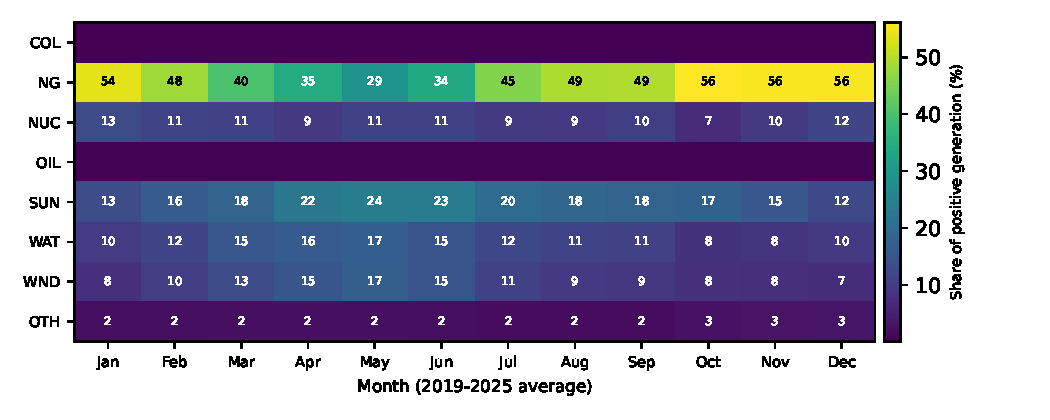
\includegraphics[width=\columnwidth]{figures/fig_fuel_mix.pdf}
\caption{Mean share of positive generation by fuel and month, 2019-2025, from the raw EIA-930 fuel-type file over the 53,416 hours with all eight non-geothermal fuels reported. Numbers are percentages.}
\label{fig:fuelmix}
\end{figure}

\begin{figure}[t]
\centering
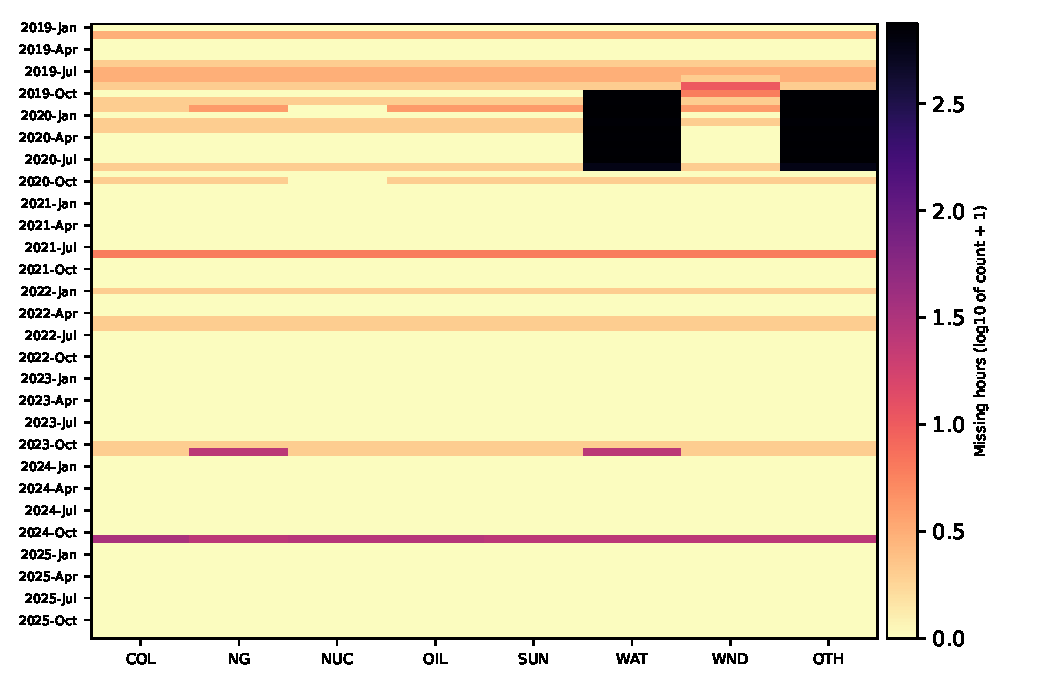
\includegraphics[width=\columnwidth]{figures/fig_missing.pdf}
\caption{Missing fuel-type hours by month and fuel, 2019-2025, on the complete hourly UTC grid. Colour is log scale. Geothermal is omitted (missing in 99.4\% of hours).}
\label{fig:missing}
\end{figure}

\subsection{Time base}
The pipeline stores all timestamps in UTC on a complete hourly grid from 2019-01-01 00:00 to 2025-12-31 23:00, which is 61,368 hours. Local time in the Pacific zone is stored in a separate column, along with a flag for daylight saving hours. Local time is used only for calendar features and for defining local days. Of the 61,272 rows in the headline table, 39,944 fall in Pacific daylight saving time. Storing UTC avoids the duplicated and missing hours that occur at daylight saving transitions, and the complete grid makes missing hours explicit.

\section{Methods}
\label{sec:methods}

\subsection{Design decisions}
Table~\ref{tab:decisions} lists the main decisions, the alternatives that were on the table, and the reasons for each choice. Where a decision came from the team, the date of confirmation is given. The decisions are recorded in the project checklists, so they can be traced.

\begin{table*}[t]
\caption{Main design decisions, alternatives, and reasons.}
\label{tab:decisions}
\centering
\small
\begin{tabular}{@{}p{2.8cm}p{3.6cm}p{3.6cm}p{5.4cm}@{}}
\toprule
Decision & Chosen & Alternative considered & Reason and status \\
\midrule
Balancing authority & CAISO only & 6 to 8 authorities (proposal) & Team decision, 2026-11-18. The proposal has not been updated. \\
Headline horizon & 7 days ahead & Next hour, 6 hours, 24 hours (PERT) & Planning use. Team decision, 2026-11-18. The 1-hour model is a secondary check. \\
Time base & UTC storage with local-time column & Local time throughout (proposal) & Avoids duplicated and missing hours at daylight saving transitions. Follows the data management plan. \\
Short gaps & Linear interpolation up to 3 hours, flagged & PUDL imputation method & Demand is missing only about 24 hours, so the simpler method was judged adequate. \\
Sparse days & Drop a day if more than 10\% of CI hours are missing & Require every fuel present (drops 332 days) & The hydro-only exception was confirmed by the team on 2026-11-18. \\
Hydro gaps & Keep CI where only hydro is missing; flag & Drop those hours & Avoids losing about 330 days of data under the stricter rule. Biases CI upward slightly. Team decision, 2026-11-18. \\
Solar weather driver & Dropped & Solar irradiance from another source & NOAA stations do not report solar. Team decision, 2026-11-18. \\
Weather in 7-day model & None & Observed weather & Observed weather would leak the future into the forecast. \\
Weather in 1-hour model & Hourly observed temperature and wind, lagged & Daily weather & Only the hour before each forecast is known in advance. Tested; does not help. \\
Station weights & Equal, 0.2 per station & Load-weighted & Team decision, 2026-11-18. Not load-weighted, which is listed as a limitation. \\
Outliers & Flag, never delete & Remove & Preserves the record and lets users choose their own handling. \\
Carbon intensity target & Lifecycle (headline); combustion-only (sensitivity) & Lifecycle only & Shows how the choice of definition affects results. \\
Model & Gradient boosting, untuned & Other families & Baseline for comparison. No other family was compared. \\
Evaluation & Rolling origin (headline); fixed split (diagnostic) & Fixed split only & The fixed split alone gives a misleading picture (Section~\ref{sec:results}). \\
\bottomrule
\end{tabular}
\end{table*}

\subsection{Revisions during the project}
The frozen tables went through several revisions in one working day, and each revision is traceable through its manifest. Table~\ref{tab:revisions} lists them. The first build kept 53,400 of the 61,368 grid hours. The difference is 7,968 hours, which is exactly 332 days, and it matches the stricter every-fuel rule described in Section~\ref{sec:methods}. The later builds keep all 61,272 hours after the sparse-day rule. Earlier tables are superseded, and they are kept only so that the history can be audited.

\begin{table*}[t]
\caption{Revisions of the frozen tables, from the table manifests.}
\label{tab:revisions}
\centering
\small
\begin{tabular}{@{}p{2.2cm}p{2.0cm}rrp{6.0cm}@{}}
\toprule
Table & Built (UTC) & Rows & Features & Change \\
\midrule
v0.1.0 & 22:55 & 53,400 & 27 & First build; every-fuel CI rule; 332 days dropped \\
h168 v0.2.0 & 23:21 & 61,272 & 26 & Hydro rule adopted; 7-day horizon \\
h1 v0.2.0 & 23:21 & 61,272 & 27 & 1-hour table with daily weather \\
h1 v0.3.0 & 23:40 & 61,272 & 28 & Hourly weather replaces daily weather \\
h168 v0.3.0 & 23:44 & 61,272 & 26 & Adds three weather-flag columns; headline table \\
\bottomrule
\end{tabular}
\end{table*}

\subsection{Pipeline design and reproducibility}
The pipeline runs as one command that reads the raw files and writes a Parquet feature table, a manifest, and a copy of the manifest in the reports folder. The manifest records the SHA-256 checksum of the table, the list of features and targets, the split dates and row counts, the days dropped by the sparse-day rule, the results of the no-future check, and the model results. A separate loader verifies the checksum before it returns the table to a teammate. Two frozen tables were built: a headline table for the 7-day horizon with 26 features, and a secondary table for the 1-hour horizon with 28 features. Four of the 1-hour features are hourly weather features.

Reproducing the tables needs the raw files, which are not in the repository. Reproduction proceeds in four steps: restore the raw files and confirm their checksums against the raw manifest; run the pipeline for each horizon with the tag and date range recorded in the manifest; run the loader check on each output table; and run the test suite. The software environment is pinned in a requirements file. Two Python environments were used for verification: a project environment and a PUDL environment that holds the Catalyst Cooperative package. Their pandas and pyarrow versions differ, and this difference caused a real failure, described in Section~\ref{sec:learn}.

\subsection{Pipeline walkthrough}
The pipeline runs in stages, and each stage writes an intermediate result that the next stage reads. Acquisition downloads the raw files, records each file's checksum and source address, and makes the file read-only. The inventory stage counts missing and negative values by series and station, and it compares generation with nameplate capacity. The loading stage places the fuel-type data on the complete hourly grid, with one series per fuel, and it loads demand and interchange. The cleaning stage fills short gaps and flags every filled value, applies the sparse-day rule, flags negative and above-nameplate values without deleting them, and adds the local-time and daylight-saving columns. The carbon intensity stage computes the lifecycle target and the combustion-only sensitivity from the cleaned generation and the factor tables. The weather stage, which feeds only the 1-hour model, averages the five stations, fills gaps with climatology, and flags filled values. The feature stage builds the 7-day features, which are shifted so that every input is at least a week old, and the 1-hour features, which use only values before each hour. The split stage assigns each row to train, validate, or test and lists the weekly origins for rolling evaluation. The check stage runs the no-future test and its positive control on sampled timestamps and records both results in the manifest. The output stage writes the Parquet table, computes its checksum, and writes the manifest and a copy to the reports folder. For the headline build it also runs the fixed-split and rolling-origin evaluations. A final step fits and saves the demonstration models with a model card. A loader and a separate check command let teammates verify a table before using it.

\subsection{Row accounting and output contract}
Every row count in the pipeline can be traced. Table~\ref{tab:rows} shows the path from the complete grid to the splits. The headline table keeps every row that remains after the sparse-day rule, including rows whose features are incomplete. Those rows are dropped per model, not in the table.

\begin{table*}[t]
\caption{Row accounting for the headline table.}
\label{tab:rows}
\centering
\small
\begin{tabular}{@{}lr@{}}
\toprule
Stage & Hours \\
\midrule
Complete UTC hourly grid, 2019-2025 & 61,368 \\
Less four sparse days (96 hours) & $-96$ \\
Rows in the headline table & 61,272 \\
\quad Train (2019-2023) & 43,800 \\
\quad Validate (January-June 2024) & 4,368 \\
\quad Test (July 2024-December 2025) & 13,104 \\
\bottomrule
\end{tabular}
\end{table*}

Teammates use the table through its contract, which is stated in the manifest and checked by the loader. The table is indexed by UTC timestamp and has one row per hour. Its columns fall into five groups. The first group holds the two targets, the lifecycle and combustion-only CI. The second holds the feature columns listed in Table~\ref{tab:features}. The third holds the split label. The fourth holds the baseline columns used in the evaluation. The fifth holds the flags and coverage columns: a flag for each interpolated value by fuel and for demand; a flag for each negative or above-nameplate value by fuel; a flag where CI was kept without hydro; a flag and a coverage value for CI; a local-time column and a daylight-saving flag; and, in the 1-hour table, flags for each filled weather value. Downstream users should filter or report on these flags, and they must not recompute features from data after the timestamp they describe.

\subsection{Carbon intensity target}
For each hour $t$, the carbon intensity is
\begin{equation}
\mathrm{CI}(t) = \frac{\sum_{f \in F} \max\bigl(g_f(t), 0\bigr)\, e_f}{\sum_{f \in F} \max\bigl(g_f(t), 0\bigr)},
\end{equation}
where $g_f(t)$ is generation from fuel $f$ in megawatt-hours, $e_f$ is the emission factor for that fuel in gCO$_2$eq/kWh, and $F$ is the set of fuels with a factor. Negative generation is clipped to zero, since negative values are reporting artifacts or consumption. The set $F$ includes coal, natural gas, nuclear, hydro, wind, and solar. Geothermal, oil, and OTH are excluded for the reasons in Section~\ref{sec:data}.

The lifecycle factors are coal 820, gas combined cycle 490, nuclear 12, hydro 24, wind 11, and solar 48 gCO$_2$eq/kWh. They were checked against the IPCC AR5 medians as reproduced on a public encyclopedia page \cite{wikilca}. The primary IPCC annex could not be retrieved, because the server returned HTTP 403 for the addresses tried. The check is therefore against a secondary reproduction, and the report says so. Oil is not in the AR5 median table, so it is excluded from the lifecycle target. An earlier oil value was removed for this reason.

The combustion-only sensitivity factors are coal 993, gas 398, and oil 778, with zero for nuclear and renewables. These come from assumed heat rates multiplied by the default carbon dioxide content per unit of fuel energy in the IPCC 2006 guidelines \cite{ipcc2006}. They are assumptions, not values from a published table of factors, and combustion-only results are presented as a sensitivity analysis.

CI is computed only when every required fuel has a value after imputation. Hydro is the exception: when hydro is the only missing fuel, CI is kept and the hour is flagged. A first version of the rule required every fuel and dropped 332 days, mostly in 2019 and 2020. The team confirmed the hydro rule on 2026-11-18. The rule biases CI slightly upward, because hydro is low-carbon, and the size of the bias has not been quantified. The test period has no hydro gaps, so the reported test results are not affected.

\subsection{Cleaning, imputation, and flags}
Gaps of up to three consecutive hours are filled by linear interpolation, separately for each fuel and for demand. Each interpolated value is flagged. Longer gaps stay missing. A day is dropped if more than 10\% of its CI hours are missing. Four days were dropped under the final hydro rule: 2023-11-10, 2024-11-02, 2024-11-03, and 2024-11-08. Two of these fall inside the EIA fuel-type gap described in Section~\ref{sec:data}. Outliers are flagged and never deleted. The flags cover negative generation for each fuel and generation above nameplate capacity.

The four dropped days are listed in Table~\ref{tab:dropped}. Two of them overlap the EIA fuel-type gap. The causes of the other two have not been investigated.

\begin{table*}[t]
\caption{Days dropped by the sparse-day rule under the final hydro rule (96 hourly rows in total).}
\label{tab:dropped}
\centering
\small
\begin{tabular}{@{}p{3.5cm}p{4.5cm}p{7.0cm}@{}}
\toprule
Date (UTC) & Overlaps EIA gap & Note \\
\midrule
2023-11-10 & No & Cause not yet investigated \\
2024-11-02 & Yes & Gap starts 08:00 UTC on this day \\
2024-11-03 & Yes & Gap ends 07:00 UTC on this day \\
2024-11-08 & No & Cause not yet investigated \\
\bottomrule
\end{tabular}
\end{table*}

\subsection{Weather}
Weather enters only the secondary 1-hour model. Temperature and wind speed from the five ISD stations are averaged with equal weights of 0.2 per station. The weights are in a configuration file, which the team chose on 2026-11-18. When a station is missing, the average is renormalized over the stations that report. Gaps of up to three hours are interpolated. Longer gaps are filled with the hour-of-day climatology from before 2024, and every filled value is flagged. The 2025 source files end in late August, so late August through December 2025 (3,041 hours) is climatology-filled. The model uses only weather observed before each forecast hour: the value one hour earlier and the mean of the 24 hours before that.

The 7-day model uses no weather. A forecast made seven days ahead would need weather forecasts for the forecast week, and the project contains only observed weather. Using observed weather for the forecast week would leak information about the future into the forecast.

\subsection{Features}
Table~\ref{tab:features} groups the 26 features of the headline model and the 28 features of the secondary model. The 7-day model's inputs at forecast time $t$ are all at least 168 hours old. The CI and demand features use the same families: lagged values, a same-hour average over the previous four weeks, and rolling means and standard deviations ending a week before $t$. Calendar features at $t$ are known in advance and do not leak.

\begin{table*}[t]
\caption{Feature families in the two frozen tables.}
\label{tab:features}
\centering
\small
\begin{tabular}{@{}p{3.5cm}p{9.5cm}rr@{}}
\toprule
Family & Definition & 7-day & 1-hour \\
\midrule
CI lags & CI at 1-4 weeks back (7-day); CI at 1, 2, 24, 48, 168 h back (1-hour) & 4 & 5 \\
CI same-hour average & Mean of the same hour over the previous four weeks & 1 & 0 \\
CI rolling & Mean and standard deviation over 24 and 168 h, ending a week back; mean over 672 h (7-day). Over 6 and 24 h, ending at $t-1$ (1-hour) & 5 & 4 \\
Demand lags, average, rolling & Same families as CI, computed on demand & 10 & 9 \\
Calendar & Hour sine and cosine, day of week, month, day of year, weekend flag & 6 & 6 \\
Weather & Temperature and wind, lagged one hour and as a 24-hour mean ending at $t-1$ & 0 & 4 \\
\midrule
Total & & 26 & 28 \\
\bottomrule
\end{tabular}
\end{table*}

Rows with missing features, such as the first weeks of 2019, are kept in the table and dropped per model. In the 7-day training split, about 41,600 of 43,800 rows have complete features for the lifecycle target.

Figure~\ref{fig:corr} shows the correlations among the 26 features and the lifecycle target. The target correlates most strongly with the same-hour four-week average (r = 0.82) and the one-week lag (r = 0.78). Some feature pairs are almost identical: the largest correlation between two features is 0.996. The feature set is therefore highly redundant, which makes individual feature importances hard to interpret, although it does not by itself change the forecast.

\begin{figure}[t]
\centering
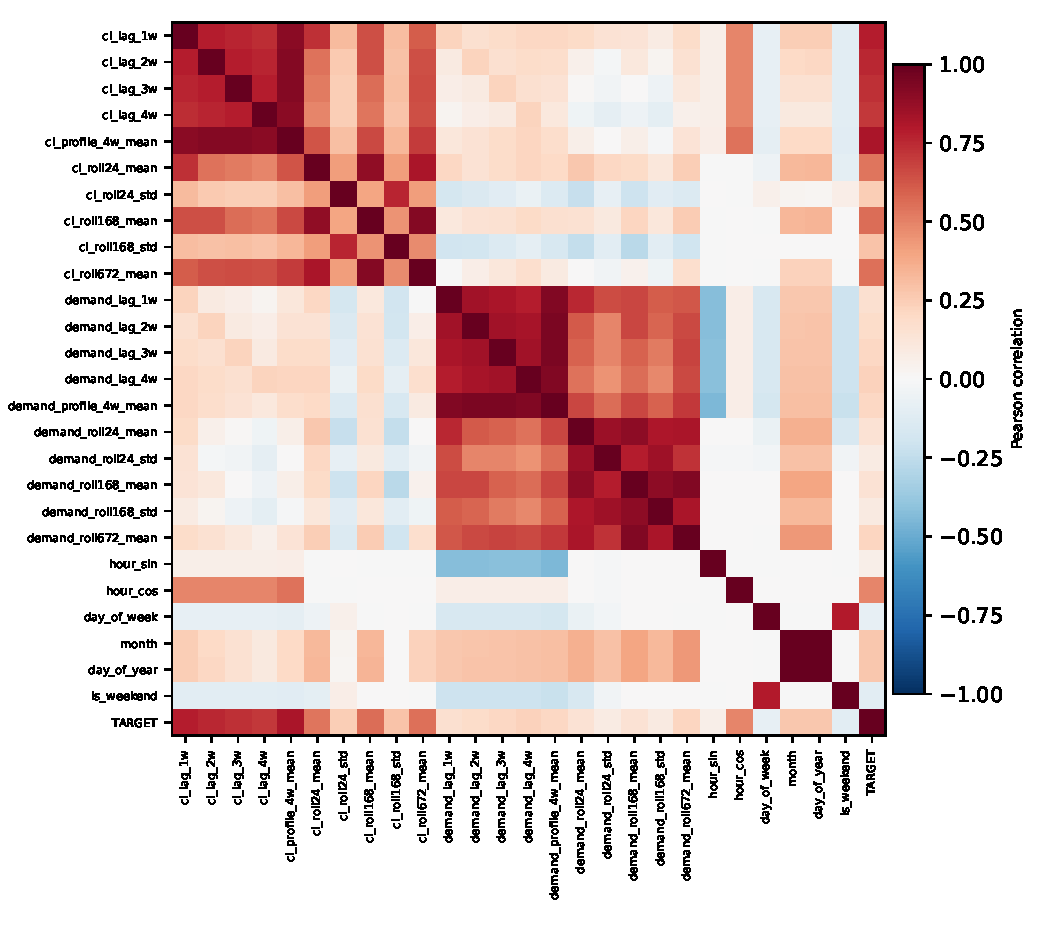
\includegraphics[width=\columnwidth]{figures/fig_feature_corr.pdf}
\caption{Pearson correlations among the 26 headline features and the lifecycle target (TARGET), from the frozen 7-day table.}
\label{fig:corr}
\end{figure}

\subsection{Splits and evaluation}
The data are split in UTC time (Table~\ref{tab:splits}). The fixed split trains on 2019-2023, validates on the first half of 2024, and tests on July 2024 through December 2025. The fixed split is a diagnostic. The headline result uses rolling origins. For the 7-day model there are 74 weekly origins across the test period. At each origin the model is refit on every row whose target is known before that origin, and it is scored on the next 168 hours. This is the approach recommended for a forecaster that is refit regularly \cite{tashman2000}.

\begin{table*}[t]
\caption{Splits and row counts in the headline table (UTC).}
\label{tab:splits}
\centering
\small
\begin{tabular}{@{}lll@{}}
\toprule
Split & Dates & Rows \\
\midrule
Train & 2019-01-01 to 2023-12-31 & 43,800 \\
Validate & 2024-01-01 to 2024-06-30 & 4,368 \\
Test & 2024-07-01 to 2025-12-31 & 13,104 \\
\bottomrule
\end{tabular}
\end{table*}

The baselines are persistence at 168 hours (the value one week earlier) and a seasonal 4-week average (the mean of the same hour in the previous four weeks). For the 1-hour model, the baseline is persistence at one hour. The headline metrics are MAE and RMSE for each target. The report also computes the regression metrics in scikit-learn's model evaluation module \cite{sklearnmetrics}: mean squared error, R-squared, explained variance, median absolute error, D2 absolute error, mean absolute percentage error, max error, root mean squared logarithmic error, and mean gamma deviance. The log-based and gamma metrics use predictions clipped at a small positive value, and no prediction needed clipping. It adds the scaled error MASE, which divides the MAE by the mean absolute error of the weekly naive forecast (value 168 hours earlier) on the training split only. The pipeline computes the extended metrics and MASE on the same 74 rolling folds and writes them to the frozen manifest. Table~\ref{tab:metrics} reports them.

\subsection{Fold-level analysis}
The pooled MAE in the headline table weights every hour equally. It does not show how consistent the advantage is from week to week. A fold-level analysis was therefore run with the same windows, baselines, and per-fold refit as the official evaluation. For each fold it records the model's MAE and the seasonal baseline's MAE. The 95\% interval for the mean per-fold difference comes from a bootstrap that resamples folds, with 5,000 resamples and a fixed random seed. Folds, rather than hours, are the resampling unit, because consecutive hours are strongly correlated and resampling hours would overstate precision. The analysis is in the project's analysis folder and writes its results to a JSON file.

\subsection{Leakage controls}
Leakage, meaning the use of information that would not have been available at prediction time, is a known source of overstated performance in data mining \cite{kaufman2012}. Two checks protect against it in this project. The no-future check takes 40 random timestamps per table. For each one, it changes every input at or after the timestamp by a large amount, and it requires that the features at that timestamp do not change. The positive control repeats the test but changes the newest input the features are allowed to use, namely the input at $t$ minus the lead time. For this control the features must change. Without the control, a check could pass because it detects nothing. Both checks pass for both tables, with 40 of 40 timestamps in each case. The unit tests check lagged and rolling features against values computed by hand, and they check that 7-day features ignore the 167 hours inside the lead window.

\subsection{Testing}
The test suite has 42 tests in eight modules. Table~\ref{tab:tests} lists the modules and what each one checks. All 42 pass in the pinned environment and in the pyenv environment used for verification.

\begin{table*}[t]
\caption{Test suite: modules, test counts, and what they check.}
\label{tab:tests}
\centering
\small
\begin{tabular}{@{}p{5.5cm}rp{9.5cm}@{}}
\toprule
Module & Tests & Checks \\
\midrule
Carbon intensity & 6 & Formula on hand-computed mixes; single-fuel case; negative generation excluded; unmapped fuels; all-missing input; renewables in the combustion-only case \\
Cleaning & 7 & Hourly grid; sparse-day rule; short-gap fill and flag; long gaps; outlier flags; DST and local time \\
Features & 6 & Lag values; no leakage at $t$; rolling windows end at $t-1$; weekend flag; index type \\
Splits & 6 & Non-overlap; train before validation; split counts; weekly rolling origins; growing training sets \\
Provenance, inventory, weather & 7 & Checksums; read-only files; manifest verification; inventory counts; area weighting; climatology fill \\
Pipeline build and no-future check & 4 & Daily climatology; weather features; no-future check and control on a synthetic series; lead features \\
Capacity and smoke test & 2 & Capacity mapping excludes storage and other balancing authorities; end-to-end build for one month \\
Saved model & 4 & Missing-value handling; save and load round trip; checksums in card; refusal on wrong checksum \\
\midrule
Total & 42 & \\
\bottomrule
\end{tabular}
\end{table*}

\subsection{Verification across environments}
The loader check and the test suite were run in three Python environments. Table~\ref{tab:envs} reports what was run and what happened. The table reports only checks that were actually run on 2026-11-20. Where a check was not run in an environment, the table says so.

\begin{table*}[t]
\caption{Verification results by environment, 2026-11-20.}
\label{tab:envs}
\centering
\small
\begin{tabular}{@{}p{3.6cm}p{3.2cm}p{4.2cm}p{3.2cm}p{2.6cm}}
\toprule
Environment & pandas, pyarrow & Tests & Loader, 7-day & Loader, 1-hour \\
\midrule
Pinned venv, from requirements.txt (Python 3.11.7) & 3.1.0, 24.0.0 & 42 pass & PASS & PASS \\
Project (pyenv, Python 3.11.7) & 3.0.3, 24.0.0 & 42 pass & PASS & PASS \\
PUDL (conda, Python 3.13) & 2.3.3, 20.0.0 & not run & PASS & PASS \\
Default Anaconda (Python 3.13.5) & 2.3.2, 19.0.0 & 38 pass (before save tests were added) & FAIL & not run \\
\bottomrule
\end{tabular}
\end{table*}

The failure in the default interpreter is raised while the Parquet file is read, so it is a reader-version problem. The file's SHA-256 checksum matches its manifest, so the file itself is intact. The project environment must therefore be pinned and tested before the tables are used.

\subsection{Saved model for demonstration}
After the evaluation, the pipeline fits both headline targets on every usable row and saves the models with a model card. The card records the SHA-256 of each file, the feature order, the training date range, and the versions of scikit-learn, NumPy, and joblib. The saved models are for demonstration only. They are trained through the end of the data, so scoring them on the test period would be circular, and the reported numbers come only from the rolling-origin evaluation. The files are compressed with joblib (compression level 3), so each is 0.53 MB. Loading a model file requires a checksum match with the card, because joblib files are Python pickles and can run code when loaded.

\section{Results}
\label{sec:results}

\subsection{Pooled 7-day results}
Table~\ref{tab:headline} reports the rolling-origin results on the test period. There are 74 weekly folds and 12,219 scored hours. Figure~\ref{fig:mae} shows the MAE values.

\begin{table*}[t]
\caption{Rolling-origin results, 7-day horizon, test period (July 2024 to December 2025). Units are gCO$_2$eq/kWh. Best model in bold.}
\label{tab:headline}
\centering
\small
\begin{tabular}{@{}llccc@{}}
\toprule
Target & Metric & Model & Seasonal 4-week & Persistence 168 h \\
\midrule
Lifecycle & MAE & \textbf{34.97} & 36.66 & 41.15 \\
 & RMSE & \textbf{45.13} & 47.47 & 53.07 \\
Combustion-only & MAE & \textbf{29.84} & 31.17 & 34.91 \\
 & RMSE & \textbf{38.55} & 40.30 & 44.96 \\
\bottomrule
\end{tabular}
\end{table*}

\begin{figure}[t]
\centering
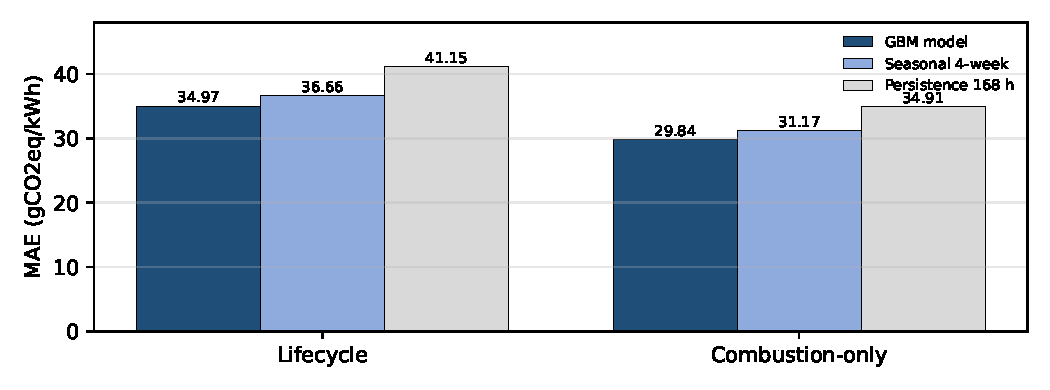
\includegraphics[width=\columnwidth]{figures/fig_mae_methods.pdf}
\caption{Rolling-origin test MAE by method and target (74 weekly folds, 12,219 hours). Values are read from the table manifest.}
\label{fig:mae}
\end{figure}

On the pooled test set, the model's lifecycle MAE is 1.69 gCO$_2$eq/kWh lower than the seasonal baseline, about 4.6\% lower. For the combustion-only target the difference is 1.33 gCO$_2$eq/kWh, about 4.3\%. These pooled differences do not show how consistent the advantage is across time, and the next subsection addresses that.

\begin{table*}[t]
\caption{Extended metrics for the 7-day rolling-origin evaluation (74 folds, 12,219 test hours). Errors in gCO$_2$eq/kWh unless stated. MASE is scaled by the training-period weekly naive error (42.12 for lifecycle, 35.80 for combustion-only). The pipeline writes these metrics into the frozen manifest. analysis/extra\_metrics.py recomputes them independently, and the values agree exactly.}
\label{tab:metrics}
\centering
\small
\begin{tabular}{@{}lrrrrrr@{}}
\toprule
 & \multicolumn{3}{c}{Lifecycle} & \multicolumn{3}{c}{Combustion-only} \\
\cmidrule(lr){2-4}\cmidrule(lr){5-7}
Metric & Model & Seasonal & Persistence & Model & Seasonal & Persistence \\
\midrule
MAE & \textbf{34.97} & 36.66 & 41.15 & \textbf{29.84} & 31.17 & 34.91 \\
RMSE & \textbf{45.13} & 47.47 & 53.07 & \textbf{38.55} & 40.30 & 44.96 \\
MSE & \textbf{2036.4} & 2253.7 & 2816.5 & \textbf{1486.4} & 1624.4 & 2021.7 \\
R-squared & \textbf{0.50} & 0.44 & 0.31 & \textbf{0.55} & 0.50 & 0.38 \\
Explained variance & \textbf{0.51} & 0.44 & 0.31 & \textbf{0.56} & 0.50 & 0.38 \\
Median absolute error & \textbf{28.13} & 28.81 & 32.54 & \textbf{23.73} & 24.62 & 27.72 \\
D2 absolute error & \textbf{0.35} & 0.32 & 0.23 & \textbf{0.39} & 0.36 & 0.28 \\
MAPE (\%) & \textbf{16.3} & 16.9 & 18.4 & \textbf{19.2} & 19.6 & 21.1 \\
Max error & \textbf{182.0} & 178.2 & 183.4 & \textbf{150.6} & 148.9 & 153.0 \\
RMSLE & \textbf{0.203} & 0.212 & 0.234 & \textbf{0.235} & 0.243 & 0.266 \\
Mean gamma deviance & \textbf{0.0395} & 0.0433 & 0.0560 & \textbf{0.0522} & 0.0564 & 0.0729 \\
MASE & \textbf{0.83} & 0.87 & 0.98 & \textbf{0.83} & 0.87 & 0.98 \\
\bottomrule
\end{tabular}
\end{table*}

\subsection{Fold-level consistency and uncertainty}
Table~\ref{tab:folds} summarizes the fold-level analysis, and Figure~\ref{fig:folds} plots the per-fold MAE of the lifecycle model and the seasonal baseline across the 74 weeks.

\begin{table*}[t]
\caption{Fold-level comparison of the GBM model with the seasonal 4-week baseline (74 weekly folds). Differences are model minus seasonal; negative values favor the model.}
\label{tab:folds}
\centering
\small
\begin{tabular}{@{}lrr@{}}
\toprule
 & Lifecycle & Combustion-only \\
\midrule
Median fold MAE, model & 32.36 & 27.30 \\
Median fold MAE, seasonal & 33.18 & 28.42 \\
Range of fold MAE, model & 14.87 to 82.12 & 13.66 to 70.29 \\
Folds where model beats seasonal & 40 of 74 & 37 of 74 \\
Mean per-fold difference & $-1.51$ & $-1.16$ \\
95\% bootstrap interval for the mean difference & $[-4.43,\ 1.32]$ & $[-3.66,\ 1.20]$ \\
\bottomrule
\end{tabular}
\end{table*}

\begin{figure}[t]
\centering
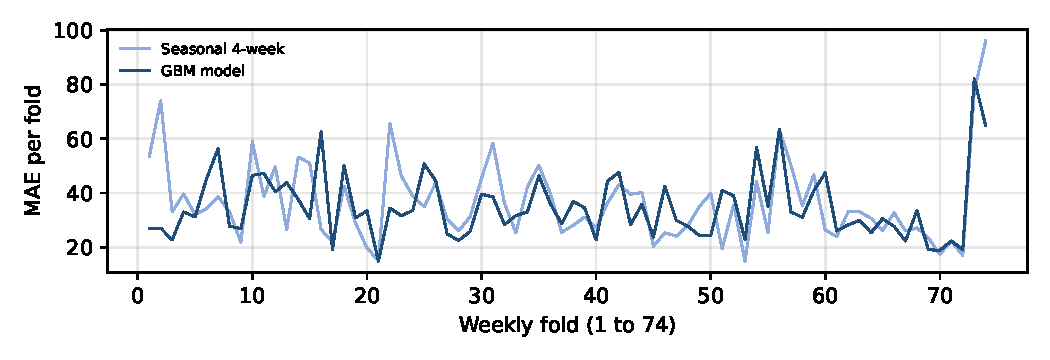
\includegraphics[width=\columnwidth]{figures/fig_fold_mae.pdf}
\caption{Per-fold MAE for the lifecycle target across the 74 weekly test folds: the GBM model and the seasonal 4-week baseline.}
\label{fig:folds}
\end{figure}

The model's median fold MAE is lower than the seasonal baseline's, by about 0.8 gCO$_2$eq/kWh for the lifecycle target (32.36 against 33.18). However, the model wins only about half of the folds, 40 of 74 for lifecycle and 37 of 74 for combustion-only. The mean per-fold difference is also negative, but the bootstrap interval includes zero for both targets. On this evidence, the model is not reliably better than the seasonal baseline from week to week. The pooled difference of 1.69 is larger than the mean per-fold difference of 1.51 because the folds are not all the same length in scored hours (they total 12,219 hours rather than 74 times 168), and the pooled measure weights hours instead of folds. Neither measure, on its own, establishes that the model is better.

The fold-level spread is also large. Individual weeks range from about 15 to about 82 MAE for the lifecycle model. The analysis does not yet explain which weeks produce the largest errors, and that is future work.

\subsection{Stability across the test period}
The advantage is not evenly spread across the test period. Table~\ref{tab:subperiod} splits the folds by origin year. The 23 folds with origins in July to December 2024 show a larger mean advantage for the model, but the interval is wide and includes zero for both targets. The 51 folds with origins in 2025 show almost no difference: the model wins 26 of 51 lifecycle folds, and the mean difference is 0.53 gCO$_2$eq/kWh in the model's favor, with an interval that includes zero. On this evidence the model's advantage over the seasonal baseline comes mainly from the 2024 part of the test period, and in 2025 the two methods are close to tied. The subsets are small, so these intervals are themselves uncertain. The subperiod results were produced by a saved script that reads the fold results and uses a fixed seed.

\begin{table*}[t]
\caption{Model minus seasonal 4-week baseline, by origin year. Negative values favor the model. Intervals are 95\% bootstrap intervals over folds.}
\label{tab:subperiod}
\centering
\small
\begin{tabular}{@{}lrrrr@{}}
\toprule
Origins & Folds & Wins (lifecycle) & Mean diff, lifecycle & Mean diff, combustion \\
\midrule
2024 (Jul-Dec) & 23 & 14 & $-3.67$ $[-11.07,\ 3.85]$ & $-3.26$ $[-9.59,\ 2.96]$ \\
2025 & 51 & 26 & $-0.53$ $[-3.20,\ 2.03]$ & $-0.21$ $[-2.46,\ 1.99]$ \\
All & 74 & 40 & $-1.51$ $[-4.43,\ 1.32]$ & $-1.16$ $[-3.66,\ 1.20]$ \\
\bottomrule
\end{tabular}
\end{table*}

\subsection{Best and worst weeks}
Table~\ref{tab:weeks} lists the three weeks where the model did best and the three where it did worst, identified by origin date. The range is wide. In the best week, the model's MAE is 14.87 against 15.16 for the seasonal baseline, a small advantage. In the worst week the model's MAE is 82.12 against 77.24 for the seasonal baseline, and in several weeks the model is far worse than the baseline. The largest advantage for the model is in the week of 2024-07-08, where its MAE is 46.9 lower than the seasonal baseline. The largest disadvantage is in the week of 2024-10-14, where the model's MAE is 62.63 against 26.61 for the seasonal baseline, 36.0 higher. The causes of the large errors have not been investigated. The table is a reminder that a mean across weeks hides wide swings, and that the swings matter to anyone who acts on a single forecast.

\begin{table*}[t]
\caption{Best and worst weekly folds for the lifecycle target, by model MAE (gCO$_2$eq/kWh). Origin is the first forecast hour of the week.}
\label{tab:weeks}
\centering
\small
\begin{tabular}{@{}lrrr@{}}
\toprule
Origin (UTC) & Model & Seasonal 4-week & Persistence 168 h \\
\midrule
2024-12-16 & 14.87 & 15.16 & 26.44 \\
2025-11-24 & 18.92 & 17.39 & 24.05 \\
2025-11-17 & 19.08 & 23.42 & 22.81 \\
\midrule
2025-08-18 & 63.55 & 63.36 & 67.09 \\
2025-12-22 & 64.84 & 96.13 & 54.66 \\
2025-12-15 & 82.12 & 77.24 & 70.42 \\
\bottomrule
\end{tabular}
\end{table*}

\subsection{Fixed split and the value of retraining}
A single fit on the training period, evaluated on the test period, gives an MAE of 39.94 for the lifecycle target and 33.94 for the combustion-only target. The seasonal baseline gives 36.77 and 31.26 on the same rows. The single fit is therefore worse than the seasonal average. On the validation period, January to June 2024, the fixed-split lifecycle model gives an MAE of 34.58. The single fit shows that the relationship between the features and CI changes over the test period, and that a model must be refit to keep pace. The rolling result is the one reported, and it is the one that should be compared with the baseline.

\subsection{Secondary 1-hour results}
The 1-hour model is fit once on the training period. On the test period, it gives an MAE of 11.42 for the lifecycle target and 10.43 for the combustion-only target. The corresponding one-hour persistence values are 11.80 and 10.85. These values are far lower than for the 7-day model because CI changes slowly from one hour to the next, so the most recent value is already a good forecast. The numbers should not be read as evidence that the 1-hour forecast is more useful than the 7-day forecast.

Hourly weather does not improve the 1-hour model. With the hourly weather features the test MAE is 11.42, and with the earlier daily-weather version it was 11.36. On the rows with observed weather, the MAE is 11.56. The result is reported as tested and not helpful for CI forecasting in this setting.

\subsection{Hydro sensitivity}
The hydro rule affects only training. The 7,907 hydro-missing hours are all in 2019 and 2020. The test period has no hydro gaps, so the test metrics are unchanged by the rule. The direction of the effect is known, and its size is not. Quantifying it would need a sensitivity run that handles hydro-only hours differently in the training data.

\subsection{One week of carbon intensity}
Figure~\ref{fig:week} shows one week of lifecycle CI in the test period. The figure plots the target itself, not a model output, and it shows the scale and variability the model must track.

\begin{figure}[t]
\centering
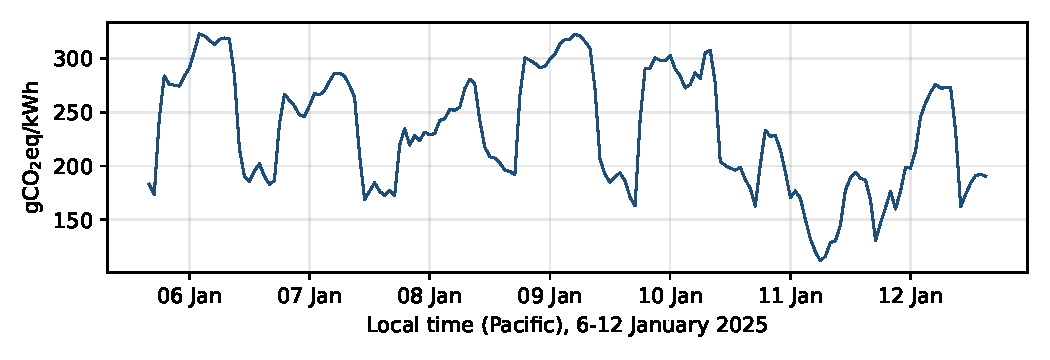
\includegraphics[width=\columnwidth]{figures/fig_ci_week.pdf}
\caption{Lifecycle carbon intensity for 6-12 January 2025, in local Pacific time, from the frozen 7-day table.}
\label{fig:week}
\end{figure}

\subsection{Daily and seasonal pattern}
Figure~\ref{fig:heat} is an exploratory view of the target over all seven years. Each cell is the mean lifecycle CI for one local hour and one calendar month, averaged across 2019-2025. The values range from about 131 to about 353 gCO$_2$eq/kWh across cells. The lowest cells fall around midday in April and May, and the highest fall from October through December, during the evening and night hours and into the early morning. Winter nights are also high. The figure is a description of the target, not a model result.

The midday minimum in spring is consistent with high midday solar output, which is part of the fuel mix. The figure alone does not establish that cause. The monthly fuel-mix breakdown (Figure~\ref{fig:fuelmix}) is consistent with it: solar's share is highest in May and gas's is lowest then. An hour-by-month fuel-mix breakdown, which would test the cause directly, has not been built. The pattern matters for the forecast because the 7-day model's seasonal features and same-hour average are designed to capture exactly this kind of repeating daily and seasonal structure.

\begin{figure}[t]
\centering
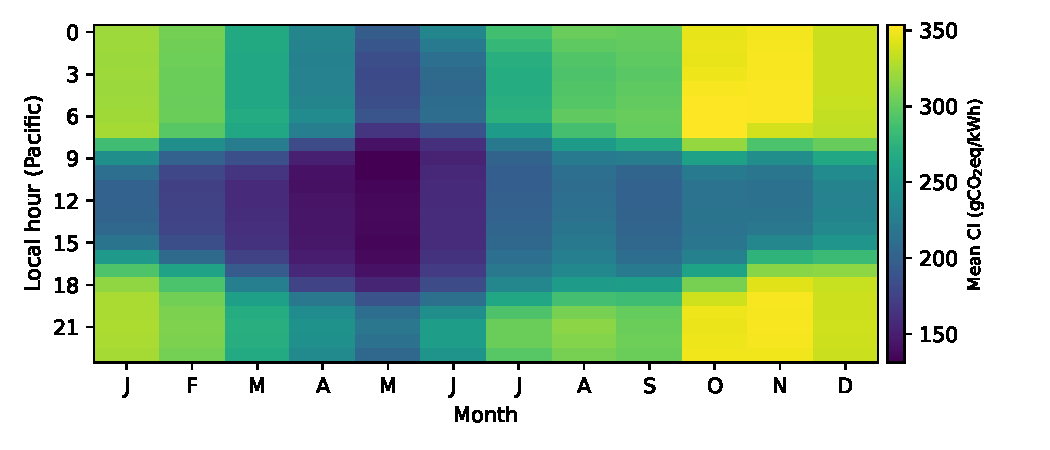
\includegraphics[width=\columnwidth]{figures/fig_ci_heatmap.pdf}
\caption{Mean lifecycle carbon intensity by local hour (Pacific) and month, 2019-2025, from the frozen 7-day table.}
\label{fig:heat}
\end{figure}

\section{Discussion}
\label{sec:discussion}

The main finding is a qualified one. A gradient boosting model with lagged and calendar features, refit weekly, has a lower pooled MAE and a lower median weekly MAE than a seasonal 4-week average on the 2024-2025 test period. The advantage is about 4 to 5\% pooled. It is not consistent across weeks: the model wins about half the folds, and the interval for the mean weekly difference includes zero. The advantage is concentrated in the 2024 folds, and in 2025 the two methods are close to tied. The report therefore does not claim that the model reliably beats the seasonal baseline. A fair summary is that the model is competitive with a strong naive baseline, and that any claimed improvement needs the fold-level evidence beside it.

Three further findings matter more for the team than the headline number. First, the naive baselines are strong. A seasonal average is a credible forecast for this target, and any gain must be measured against it on the same rows and folds. Second, retraining is necessary. A model fit once and left alone is worse than the seasonal average over the 18-month test period that follows its training data. Third, the 1-hour result is misleading if it is read on its own. It shows that CI is persistent, and it does not show that a short-horizon forecast is the right product.

The weather result is a negative finding, and it is worth stating. Temperature and wind are known drivers of demand and of the generation mix, but the hourly weather features did not improve the 1-hour model. Possible reasons include the equal station weights, which do not reflect load, the climatology fill for late 2025, and the fact that the lagged CI and demand features already carry most of the signal at a one-hour horizon. These explanations have not been tested. The project also did not test whether weather helps a 7-day forecast, because no forecast weather is available.

Some of the most useful work in this project was the work that produced negative or uncomfortable results. The fixed split, the fold-level analysis, and the weather test each changed what could honestly be claimed. A pipeline that reported only its best number would have made the advantage look firmer than the evidence supports.

\subsection{Implications for the modeling work}
The findings have practical implications for the M2 and M3 modeling work, and the handoff is written to support them. Any model should be compared with the seasonal 4-week average on the same folds, and its difference should be reported with a fold-level interval, not only as a pooled MAE. A model should be refit at each weekly origin, because the fixed fit is worse than the baseline. The 7-day model should not use weather, since no forecast weather is available. The 1-hour table should be used as a sanity check rather than as evidence of forecast value. Any model that uses the hydro-missing hours should report whether those hours affect its results, and the flags in the table allow that check. These recommendations follow directly from the results above and do not depend on the choice of model family.

\section{Threats to Validity}
\label{sec:threats}

\subsection{Internal validity}
The main internal risk is leakage. The no-future check and the positive control address it, and the unit tests check the lag and rolling features by hand. A residual risk remains in the choices made from the data: the sparse-day rule, the interpolation limit, and the hydro rule were set before the final evaluation, but they were chosen after the inventory revealed the problems they address. These choices do not use the test period's values, but they were informed by the full dataset, including the test years. Its size is unknown, and it cannot be measured without a separate holdout period.

\subsection{External validity}
The results cover one balancing authority, one weather network of five airports, and one test period of 18 months. The seasonal baseline is strong in this period, and a different period could show a larger or smaller margin. The results should not be transferred to other grids.

\subsection{Construct validity}
The target is a model of lifecycle CI built from medians reproduced from a secondary source, and from combustion factors that are assumptions. The metrics are two scale-dependent errors. A user who cares about the frequency of cleaner hours, or about the cost of a wrong decision, would need different measures. The report does not address those.

\section{Process and Team Coordination}
\label{sec:process}
The project was run from a checklist, with one checklist for the team and one for my individual coding tasks. Each team decision is recorded with the date it was confirmed. The main dated milestones are these.
\begin{itemize}
\item \textbf{2026-11-18 (day 28 of 37 in the project plan).} The team confirmed the 7-day horizon, the hydro rule, and dropping the solar driver. The raw data were downloaded and checksummed, the EIA and NOAA keys were tested, and the first test suite passed.
\item \textbf{2026-11-18 to 2026-11-20.} Inventory and coverage reports were saved, the frozen tables were rebuilt and checked, and the rolling-origin evaluation was run. The saved demonstration models were built, and the fold-level analysis was added after the first report draft.
\item \textbf{2026-12-01.} Final submission.
\end{itemize}
Coordination with the teammates happened through the checklists and a shared handoff. The loader is the handoff point for the M2 and M3 modeling work, and a teammate's confirmation that they can load the table is still open. The project did not use one-week sprints, a sprint board, or meeting minutes, and no pair programming session is recorded. These are gaps against the course requirements, and they are listed in Appendix~A with the actions needed. The report does not claim that they were done.

\section{Key Learnings, Technical Difficulties, and Best Practices}
\label{sec:learn}

\subsection{Key learnings}
The first learning is that the evaluation design matters as much as the model. The fixed split and the rolling-origin result gave different answers about whether the model beat the baseline. Reporting both makes the difference visible. The fold-level analysis then showed that even the rolling result is less clear than the pooled number suggests.

The second learning is that a leakage check needs a positive control. A check that only confirms features do not change when future inputs change can pass for a pipeline that detects nothing. The positive control requires features to change when a legitimately available input changes, so the check can fail when it should.

The third learning is that source data must be inspected before it is trusted. Four separate issues surfaced only in the inventory step: the 24-hour EIA gap, the solar negative values, the geothermal and OTH coverage, and the station-name mismatch. None would have been visible in a model's error metrics, and each would have changed a result if left unhandled.

The fourth learning concerns the cost of a strict rule. Requiring every fuel to be present for CI dropped 332 days, and keeping CI when only hydro is missing dropped four days. The change is defensible, but it is a decision with a bias, and it must be documented as one.

The fifth learning is that uncertainty should be reported with the headline number. A pooled MAE and a fold-level interval can tell different stories. Reporting only the pooled number would have overstated the case.

\subsection{Technical difficulties}
The main difficulties were the following.
\begin{itemize}
\item \textbf{Environment mismatch.} The PUDL environment used pandas 2.3.3 and pyarrow 20.0.0, and the project environment used pandas 3.1.0 and pyarrow 24.0.0. A table written by pyarrow 24 could not be read by pyarrow 19, which is the version in the default Anaconda interpreter on the same machine. The loader check failed there with a repetition-level histogram error. The fix was to run the check in an environment whose versions match the writer's, and to document each environment's versions in the provenance notes. The requirements file pins the versions of a clean virtual environment, which was built and checked on 2026-11-20; in that environment the frozen table is reproduced exactly.
\item \textbf{Checksum traceability.} The checksum recorded in the checklist for an earlier 7-day build does not match the checksum in the stored manifest for the v0.2.0 table, which is different again. The v0.3.0 table adds three weather-flag columns to the 7-day table, and the values in every shared column are identical. A rebuild of v0.3.0 from the raw files in the pinned environment reproduces its checksum exactly, and the rebuild used a scratch output that was deleted afterwards. The cause of the earlier checklist value has not been identified.
\item \textbf{Library version changes results.} The same code and data gave a headline lifecycle MAE of 35.22 under scikit-learn 1.9.1 and 34.97 under the pinned 1.6.1. The gradient boosting fit depends on the library version. Every model number in this report was therefore recomputed in the pinned environment, and the earlier fold results from the 1.9.1 environment were replaced.
\item \textbf{Station identity.} The GHCN identifier for the Sacramento series refers to an airport that is not the one most readers would expect. Checking the WBAN identifier, rather than trusting the name, resolved it.
\item \textbf{Pagination and access.} EIA downloads were paginated, and the NOAA hourly files come from a public bucket. Some reference pages returned HTTP 403 when fetched automatically, so the primary emission-factor document could not be read.
\item \textbf{Mixed-length folds.} The fold lengths in scored hours are not all 168, so per-fold and pooled averages are not the same. Reporting only one of them would have hidden this.
\end{itemize}

\subsection{Best practices}
The practices I would keep are these.
\begin{itemize}
\item Keep raw data read-only and record a checksum for each file at acquisition, then verify the checksums before every build.
\item Keep keys out of code and out of manifests. The source addresses in the manifest were written without the API keys, and a scan of the project for key values found none.
\item Flag rather than delete. Every imputed value, outlier, and filled weather value carries a flag so that a user can exclude or report it.
\item Build the baseline before the model, and report the baseline on the same rows and folds as the model.
\item Pair each leakage check with a positive control.
\item Report pooled and fold-level results together, with an interval on the difference.
\item Write each decision that changes results into the record with a date and an owner.
\end{itemize}

\section{Limitations and Future Work}
\label{sec:limits}

The limitations are listed so that a reader can weigh the results correctly.
\begin{itemize}
\item \textbf{Scope.} One balancing authority (CAISO) and one weather network. The project proposal named six to eight balancing authorities, and the team reduced the scope to CAISO. The proposal has not yet been updated to match.
\item \textbf{Weather.} The station weights are equal, so the averages do not reflect population or load. Hourly weather is missing from late August 2025, and climatology fills it. The 7-day model has no weather at all.
\item \textbf{Solar.} Solar generation is in the fuel mix, but the project has no solar irradiance driver. NOAA does not provide solar radiation for these stations.
\item \textbf{Emission factors.} The lifecycle factors were checked against a secondary reproduction of the IPCC medians, not the primary annex. The combustion-only factors are assumptions.
\item \textbf{Hydro.} The hydro rule keeps CI in hydro-missing hours, which biases CI slightly upward. The bias is not quantified.
\item \textbf{Demand.} Demand gaps are filled by three-hour interpolation rather than the PUDL method.
\item \textbf{Model.} The gradient boosting model is untuned, and no other model family was compared. The advantage over the seasonal baseline is small and not reliable across folds.
\item \textbf{Metrics.} The extended metrics and MASE are written into the frozen manifest. MASE uses a training-period scale, so it is only meaningful for this horizon and this training window.
\item \textbf{Comparison with published work.} The results are compared qualitatively with four published forecasts (Section~\ref{sec:related}). No like-for-like comparison has been run.
\end{itemize}

Future work, in priority order: (1) test whether the model's advantage holds under a different baseline, a longer test period, and a second balancing authority; (2) identify the weeks with the largest errors and explain them with the fuel mix; (3) quantify the hydro bias with a sensitivity run; (4) retrieve and check the primary IPCC annex; (5) run a published method on the same data and folds for a like-for-like comparison; and (6) release the data with a datasheet after the license terms for EIA, NOAA, and PUDL are confirmed.

\section{Considerations for Use}
\label{sec:considerations}
A carbon intensity forecast can influence when people run flexible loads, so its errors have consequences. The test-period MAE of about 35 gCO$_2$eq/kWh should be read against the range of CI values shown in Figure~\ref{fig:week}, not as a stand-alone accuracy claim. A user who schedules around a forecast should also know that the result depends on the definition: lifecycle and combustion-only values differ, and the lifecycle factors are medians from a secondary reproduction. Any published number should state its definition.

The fold-level result has a practical consequence. A forecast that is only marginally better than a seasonal average on average, and not better in about half of the weeks, is useful as a benchmark but should not be presented as a substantial improvement. Overstating a small margin would give users confidence the evidence does not support. The report therefore states the uncertainty alongside every headline figure.

The project uses public data and holds no personal information. Its main obligations are to cite the data sources accurately, to confirm the license terms before any public release, and to keep API keys out of shared files.

\section{Relation to the Course}
\label{sec:course}

Table~\ref{tab:course} maps the main course topics the project exercises to the place in this report where each is addressed. The mapping is by topic; the course learning outcomes themselves are not restated here. The project exercises course methods rather than new model families. The data management work covers acquisition, provenance, checksums, read-only storage, and documented decisions. The time-series work covers time-ordered splits, lagged and rolling features that respect the forecast time, and a forecast evaluated against naive baselines. The evaluation covers scale-dependent error measures, repeated forecast origins, and an uncertainty estimate on the difference from a baseline. The leakage controls and the test suite cover verification. The project does not use deep learning, recommender systems, or a user interface, because those are outside the scope of the course. Table~\ref{tab:clo} maps the project to each course learning outcome (CLO), with its status.

\begin{table*}[t]
\caption{Course topics exercised by the project, and where they appear.}
\label{tab:course}
\centering
\small
\begin{tabular}{@{}p{4.5cm}p{11.5cm}@{}}
\toprule
Topic & Where addressed \\
\midrule
Data acquisition and provenance & Section~\ref{sec:data}; checksummed manifest; read-only raw store \\
Data quality and inventory & Tables~\ref{tab:inventory} and \ref{tab:dropped}; flags for every filled or suspect value \\
Time series and time order & Section~\ref{sec:methods}, splits and rolling origins; no-future check \\
Feature engineering for forecasting & Table~\ref{tab:features}; lags and rolling windows that end before the forecast time \\
Baselines and benchmarking & Persistence and seasonal average; Table~\ref{tab:headline} \\
Evaluation metrics & MAE, RMSE, and the extended set (Table~\ref{tab:metrics}); Table~\ref{tab:folds} for uncertainty \\
Leakage and validation & Positive control; unit tests; Table~\ref{tab:tests} \\
Reproducibility and testing & Pinned environments; Table~\ref{tab:envs}; 42 tests \\
Communicating limits & Section~\ref{sec:threats}; Section~\ref{sec:limits} \\
\bottomrule
\end{tabular}
\end{table*}

\begin{table*}[t]
\caption{Course learning outcomes (CLOs) and how this report addresses them. Status is stated as of the date of this report.}
\label{tab:clo}
\centering
\small
\begin{tabular}{@{}p{1.0cm}p{5.0cm}p{2.6cm}p{7.6cm}@{}}
\toprule
CLO & Outcome (abbreviated) & Status & How this report addresses it \\
\midrule
1 & Describe ML concepts, algorithms, practices, tools, and methods & Addressed & Gradient boosting against naive baselines, leakage controls, rolling-origin evaluation, and error metrics (Sections~\ref{sec:methods} and \ref{sec:results}) \\
2 & Learn with a social purpose; apply ML to significant and sustainable problems & Addressed & Carbon intensity forecasting to support cleaner electricity use (Sections~\ref{sec:related} and \ref{sec:considerations}) \\
3 & Use Python and ML libraries & Addressed & Python with pandas, NumPy, PyArrow, scikit-learn, and pytest (Appendix~\ref{app:tools}). R was not used \\
4 & Create and implement a regression, classification, or clustering problem & Partly addressed & A regression problem with its own software pipeline and tests. The report covers the M1 part of a team project; the clustering work belongs to a teammate \\
5 & Critique current literature and present it & Partly addressed & Comparison with three published forecasts (Section~\ref{sec:related}, Table~\ref{tab:published}). A fuller literature critique and the presentation have not been done \\
6 & Explain how industry uses ML & Not addressed & The report does not discuss industry use \\
7 & Communicate ML knowledge verbally and in writing & Partly addressed & This written report. The verbal presentation has not yet been given \\
8 & Responsibly use and evaluate generative AI tools & Addressed & Generative AI use is disclosed with its purposes and how its output was checked (Section~\ref{sec:learn} and Appendix~\ref{app:tools}) \\
\bottomrule
\end{tabular}
\end{table*}

\section{Sustainability, Innovation, and Prospects}
\label{sec:sustain}

\subsection{Relation to the UN Sustainable Development Goals}
The project works toward two of the 17 UN Sustainable Development Goals (SDGs): SDG 7, affordable and clean energy, and SDG 13, climate action. Its contribution is indirect. It produces a checkable carbon intensity series and forecast for a large grid, which a user could use to shift flexible electricity use toward cleaner hours. This is the link to SDG 7 and SDG 13 described in Section~\ref{sec:considerations}. The report measures forecast accuracy, not emissions avoided. The margin over a seasonal baseline is small and not consistent from week to week (Section~\ref{sec:results}), so the project does not show that any emission reduction would follow.

\subsection{Innovation}
The novelty of the project is modest. Forecasting carbon intensity and comparing a model with naive baselines are established practices, and the model is a standard gradient boosting baseline (Section~\ref{sec:related}). The project's own contributions are narrower. They are a positive control for the leakage check, fold-level uncertainty with a split by origin year, a check that model results depend on the library version (Section~\ref{sec:learn}), and a checksummed pipeline for CAISO. None of these is a new method.

\subsection{Prospects of publication or competition}
The prospects are low in the current form. The forecast advantage over a strong seasonal baseline is small, and it is not statistically reliable from week to week. The study covers one balancing authority and one horizon, and it has no forecast weather inputs. A publishable version would need a stronger model or more regions, a like-for-like comparison with a published method (not yet done, Section~\ref{sec:related}), and forecast inputs for the weather and generation drivers that the published methods use.

\section{Conclusion}
This report described the data pipeline I built for a team forecast of California carbon intensity. The pipeline converts raw hourly grid and weather data into a checksummed feature table, enforces the rule that no feature may use future information, and produces a rolling-origin evaluation. On the 2024-2025 test period, a seasonal 4-week average is a strong baseline. The gradient boosting model improves on it by about 4 to 5\% on the pooled test set, but it wins only about half of the weekly folds, and the interval for the mean weekly difference includes zero. Retraining is necessary for the model to perform at all, and hourly weather does not help the 1-hour model. The most important practical lessons were to evaluate against strong baselines, to test leakage controls with a positive control, to inspect source data before modeling, and to report uncertainty with the headline number.

\section*{CRediT Statement}
Roles follow the Contributor Roles Taxonomy \cite{credit}. Jayanth Naga Sai Pasupulati: software, data curation, methodology, validation, investigation, and writing (original draft of the M1 section). Aryan: methodology, software, formal analysis, and validation for the carbon-intensity forecasting models (regression and gradient boosting, compared against baselines). Jaskirat: methodology, formal analysis, and software for the day-type clustering and load-shifting simulation. The roles of Aryan and Jaskirat are drafted from the team's role description, which was written as a plan before the work. Each contributor should confirm their own entry against the work actually done.

\section*{Generative AI and Tool Use}
Tools used are listed in Appendix~B. The only generative AI tools used were Claude and Claude Code (Anthropic). They were used for formatting, vocabulary, syntax, and boilerplate code. All of their output was checked by proofreading.

\section*{Data and Code Availability}
The code, tests, configuration, reports, the fold-level analysis, and the saved demonstration models are in the public repository at \url{https://github.com/ARYANM168/ML-PROJECT-DATA-245}, which was pushed on 2026-11-20. Raw data are not included, because the repository excludes them and the checksummed manifest identifies them. The frozen feature tables are available from the link in Appendix~C. The raw data sources are listed in Table~\ref{tab:sources}.

% ---------------------------------------------------------------
% References
% ---------------------------------------------------------------
\begin{thebibliography}{99}
\bibitem{ipcc2014} IPCC, \emph{Climate Change 2014: Mitigation of Climate Change}, Contribution of Working Group III to the Fifth Assessment Report, Annex III. Cambridge, U.K.: Cambridge Univ. Press, 2014.
\bibitem{ipcc2006} IPCC, \emph{2006 IPCC Guidelines for National Greenhouse Gas Inventories}, Vol. 2, Energy. Hayama, Japan: IGES, 2006.
\bibitem{wikilca} Wikipedia contributors, ``Life-cycle greenhouse gas emissions of energy sources,'' Wikipedia. [Online]. Available: \url{https://en.wikipedia.org/wiki/Life-cycle_greenhouse_gas_emissions_of_energy_sources}. Accessed Oct. 15, 2026.
\bibitem{hyndman2021} R. J. Hyndman and G. Athanasopoulos, \emph{Forecasting: Principles and Practice}, 3rd ed. Melbourne, Australia: OTexts, 2021. [Online]. Available: \url{https://otexts.com/fpp3/}
\bibitem{tashman2000} L. J. Tashman, ``Out-of-sample tests of forecasting accuracy: An analysis and review,'' \emph{Int. J. Forecasting}, vol. 16, no. 4, pp. 437-450, 2000.
\bibitem{hyndman2006} R. J. Hyndman and A. B. Koehler, ``Another look at measures of forecast accuracy,'' \emph{Int. J. Forecasting}, vol. 22, no. 4, pp. 679-688, 2006.
\bibitem{friedman2001} J. H. Friedman, ``Greedy function approximation: A gradient boosting machine,'' \emph{Ann. Statist.}, vol. 29, no. 5, pp. 1189-1232, 2001.
\bibitem{pedregosa2011} F. Pedregosa \emph{et al.}, ``Scikit-learn: Machine learning in Python,'' \emph{J. Mach. Learn. Res.}, vol. 12, pp. 2825-2830, 2011.
\bibitem{sklearnmetrics} scikit-learn developers, ``Metrics and scoring: Quantifying the quality of predictions.'' [Online]. Available: \url{https://scikit-learn.org/stable/modules/model_evaluation.html}
\bibitem{eia930} U.S. Energy Information Administration, ``EIA open data (API v2) and hourly balancing authority data.'' [Online]. Available: \url{https://www.eia.gov/opendata/}
\bibitem{pudl} Catalyst Cooperative, ``Public Utility Data Liberation (PUDL) project documentation.'' [Online]. Available: \url{https://catalystcoop-pudl.readthedocs.io/}
\bibitem{menne2012} M. J. Menne, I. Durre, R. S. Vose, B. E. Gleason, and T. G. Houston, ``An overview of the Global Historical Climatology Network-Daily database,'' \emph{J. Atmos. Ocean. Technol.}, vol. 29, no. 7, pp. 897-910, 2012.
\bibitem{smith2011} A. Smith, N. Lott, and R. Vose, ``The Integrated Surface Database: Recent developments and partnerships,'' \emph{Bull. Amer. Meteor. Soc.}, vol. 92, no. 6, pp. 704-708, 2011.
\bibitem{wilkinson2016} M. D. Wilkinson \emph{et al.}, ``The FAIR guiding principles for scientific data management and stewardship,'' \emph{Sci. Data}, vol. 3, art. no. 160018, 2016.
\bibitem{kaufman2012} S. Kaufman, S. Rosset, C. Perlich, and O. Stitelman, ``Leakage in data mining: Formulation, detection, and avoidance,'' \emph{ACM Trans. Knowl. Discov. Data}, vol. 6, no. 4, art. no. 15, 2012.
\bibitem{carboncast2022} D. Maji, P. Shenoy, and R. K. Sitaraman, ``CarbonCast: Multi-day forecasting of grid carbon intensity,'' in \emph{Proc. 9th ACM Int. Conf. Systems for Energy-Efficient Buildings, Cities, and Transportation (BuildSys '22)}, Boston, MA, USA, Nov. 2022. doi: 10.1145/3563357.3564079.
\bibitem{cleancast2023} T. Welsh, B. Hart, K. Eulau, and B. Baer, ``CleanCAst,'' MIDS Capstone Project, UC Berkeley School of Information, 2023. [Online]. Available: \url{https://www.ischool.berkeley.edu/projects/2023/cleancast}
\bibitem{leerbeck2020} K. Leerbeck \emph{et al.}, ``Short-term forecasting of CO$_2$ emission intensity in power grids by machine learning,'' arXiv:2003.05740, Mar. 2020. [Online]. Available: \url{https://arxiv.org/abs/2003.05740}
\bibitem{ensembleci2025} L. Yan, L. Wang, S. Liu, and Y. Ding, ``EnsembleCI: Ensemble learning for carbon intensity forecasting,'' in \emph{Proc. 16th ACM Int. Conf. Future and Sustainable Energy Systems (E-ENERGY '25)}, Rotterdam, The Netherlands, 2025. doi: 10.1145/3679240.3734630. arXiv:2505.01959.
\bibitem{watttime} WattTime, ``Methodology and validation: Marginal emissions.'' [Online]. Available: \url{https://www.watttime.org/marginal-emissions-methodology/}. Accessed Nov. 20, 2026.
\bibitem{radovanovic2021} A. Radovanovic \emph{et al.}, ``Carbon-aware computing for datacenters,'' arXiv:2106.11750, Jun. 2021. [Online]. Available: \url{https://arxiv.org/abs/2106.11750}
\bibitem{credit} CRediT, ``Contributor Roles Taxonomy.'' [Online]. Available: \url{https://credit.niso.org/}
\end{thebibliography}

% ---------------------------------------------------------------
% Appendices (do not count toward the 12-page minimum)
% ---------------------------------------------------------------
\appendices

\section{Rubric Criteria and Evidence}
\label{app:rubric}

The term-project rubric grades this report. Its criteria appear in the rubric's order. Status is stated as of the date of this report. ``Met'' means the evidence exists and can be checked. ``Partly met'' and ``Not yet met'' are stated as they are. The tools used to produce the evidence, including generative AI, are listed in Appendix~\ref{app:tools}.

\begin{table*}[t]
\caption{Term-project rubric (report, 43 points): criteria, status, and evidence.}
\label{tab:termrubric}
\centering
\small
\begin{tabular}{@{}p{0.35cm}p{4.0cm}p{1.8cm}p{7.2cm}@{}}
\toprule
\# & Criterion (points) & Status & Evidence and remaining work \\
\midrule
1 & Report: format, completeness, language, grammar, plagiarism, Turnitin (7) & Partly met & IEEE class (\texttt{IEEEtran}, Computer Society option). Body of 12 or more pages before the references, with appendices after. No code listings or screenshots. All 19 references are cited and each citation has an entry. Not done: Turnitin submission, a full proofread, and a plagiarism check \\
2 & Relates to sustainability (5) & Met & Section~\ref{sec:sustain} names SDG 7 and SDG 13 and explains how the work relates to them. The link is indirect, and the section says so \\
3 & Lessons learned (5) & Met & Section~\ref{sec:learn}: key learnings, technical difficulties, and best practices \\
4 & Prospects of winning competition or publication (3) & Met as an assessment & Section~\ref{sec:sustain} rates the prospects as low and gives the reasons. This is a stated assessment, not an outcome \\
5 & Innovation (5) & Met as an assessment & Section~\ref{sec:sustain} states that the novelty is modest and lists the project's narrower contributions \\
6 & Evaluation of performance (5) & Met & Section~\ref{sec:results} and Table~\ref{tab:metrics}: 13 scikit-learn regression metrics for the model and two baselines, pooled over 74 weekly folds, with fold-level intervals (Table~\ref{tab:folds}). Values are written to the frozen manifest and checked by an independent script \\
7 & Technical difficulty (7) & Met & Section~\ref{sec:learn}: environment mismatch, checksum traceability, station identity, pagination and access, mixed-length folds, and library-version dependence \\
8 & Used LaTeX (1) & Met & The report is written in LaTeX with the \texttt{IEEEtran} class and was edited in Overleaf. The \texttt{.tex} source is submitted \\
9 & Literature survey (5) & Partly met & Section~\ref{sec:related} has subsections on definitions, evaluation, models, data sources, published forecasts (four, with EnsembleCI), and marginal emissions and carbon-aware use. The 22 references are each cited, and each citation has an entry. Not yet met for criterion 1: a CAISO marginal-emissions neural-network study (Mayes et al.) could not be retrieved (HTTP 403), so it is not cited, and Electricity Maps methods are not cited; both are known gaps\\
\bottomrule
\end{tabular}
\end{table*}

\section{Tools Used}
\label{app:tools}

\begin{itemize}
\item \textbf{Programming and data:} Python 3.11 and 3.13; pandas; NumPy; PyArrow; scikit-learn (gradient boosting and metrics); joblib; matplotlib (report figures); pytest.
\item \textbf{Environments and packages:} conda; the \texttt{catalystcoop.pudl} package, version 2025.12.1, from conda-forge.
\item \textbf{Writing and typesetting:} LaTeX (IEEEtran class) and pdfLaTeX. Overleaf was used for collaborative LaTeX editing.
\item \textbf{Data sources:} EIA API v2; NOAA CDO web services; NOAA ISD public bucket (sources, not tools).
\item \textbf{Generative AI:} Claude and Claude Code (Anthropic), used for formatting, vocabulary, syntax, and boilerplate code. All output was checked by proofreading.
\item \textbf{Project management and version control:} GitHub.
\end{itemize}

\section{Files, Sizes, and Links}
\label{app:files}

The assignment asks for files of about 1 MB or less. Files that exceed this are placed on a cloud link, with their sizes stated here.

\begin{table*}[t]
\caption{Submission files and sizes.}
\label{tab:files}
\centering
\small
\begin{tabular}{@{}p{7.5cm}p{4.5cm}@{}}
\toprule
File & Size \\
\midrule
This report (PDF) & 0.41 MB \\
Slides (PDF and PPTX) & \todo{measure} \\
Saved model, lifecycle target (compressed) & 0.53 MB \\
Saved model, combustion target (compressed) & 0.53 MB \\
Model card (JSON) & 1.8 KB \\
Headline feature table (Parquet, 26 features) & 14 MB; cloud link only \\
Secondary feature table (Parquet, 28 features) & 15 MB; cloud link only \\
Raw data (288 MB) & Not submitted; identified by checksum in the manifest \\
\bottomrule
\end{tabular}
\end{table*}

The two model files are under 1 MB, so they are uploaded directly. The feature tables exceed 1 MB, so they are placed on a cloud link if they are shared at all; the raw data are not submitted.

External sources used as evidence. Each must be openable by the teaching team:
\begin{itemize}
\item Project repository: \url{https://github.com/ARYANM168/ML-PROJECT-DATA-245} (public; contains the code, tests, configuration, reports, analysis, saved models, and this report; no raw data or credentials)
\item EIA API v2 routes: \url{https://api.eia.gov/v2/electricity/rto} and \url{https://api.eia.gov/v2/electricity/operating-generator-capacity}
\item NOAA CDO web services: \url{https://www.ncei.noaa.gov/cdo-web/api/v2}
\item NOAA ISD hourly files: \url{https://noaa-global-hourly-pds.s3.amazonaws.com/}
\item CarbonCast (BuildSys 2022), DOI \url{https://doi.org/10.1145/3563357.3564079}
\item CleanCAst (UC Berkeley capstone): \url{https://www.ischool.berkeley.edu/projects/2023/cleancast}
\item Leerbeck et al. (arXiv): \url{https://arxiv.org/abs/2003.05740}
\item scikit-learn model evaluation: \url{https://scikit-learn.org/stable/modules/model_evaluation.html}
\item Emission factor reference (secondary): \url{https://en.wikipedia.org/wiki/Life-cycle_greenhouse_gas_emissions_of_energy_sources}
\end{itemize}

Not yet linked: \todo{Trello board}, if a sprint board is created; \todo{slides}, if shared.

\end{document}
